\chapter{SM}
Følgende afsnit beskriver SM'ens hardware i de enkelte blokke, grænsefladerne derimellem samt funktionen af blokkene.

\section{Overordnet design}
Nedenfor ses det overordnede hardware blokdiagram. Herefter følger en beskrivelse af de forskellige blokke samt signaler.
\begin{figure}[H]
\centering
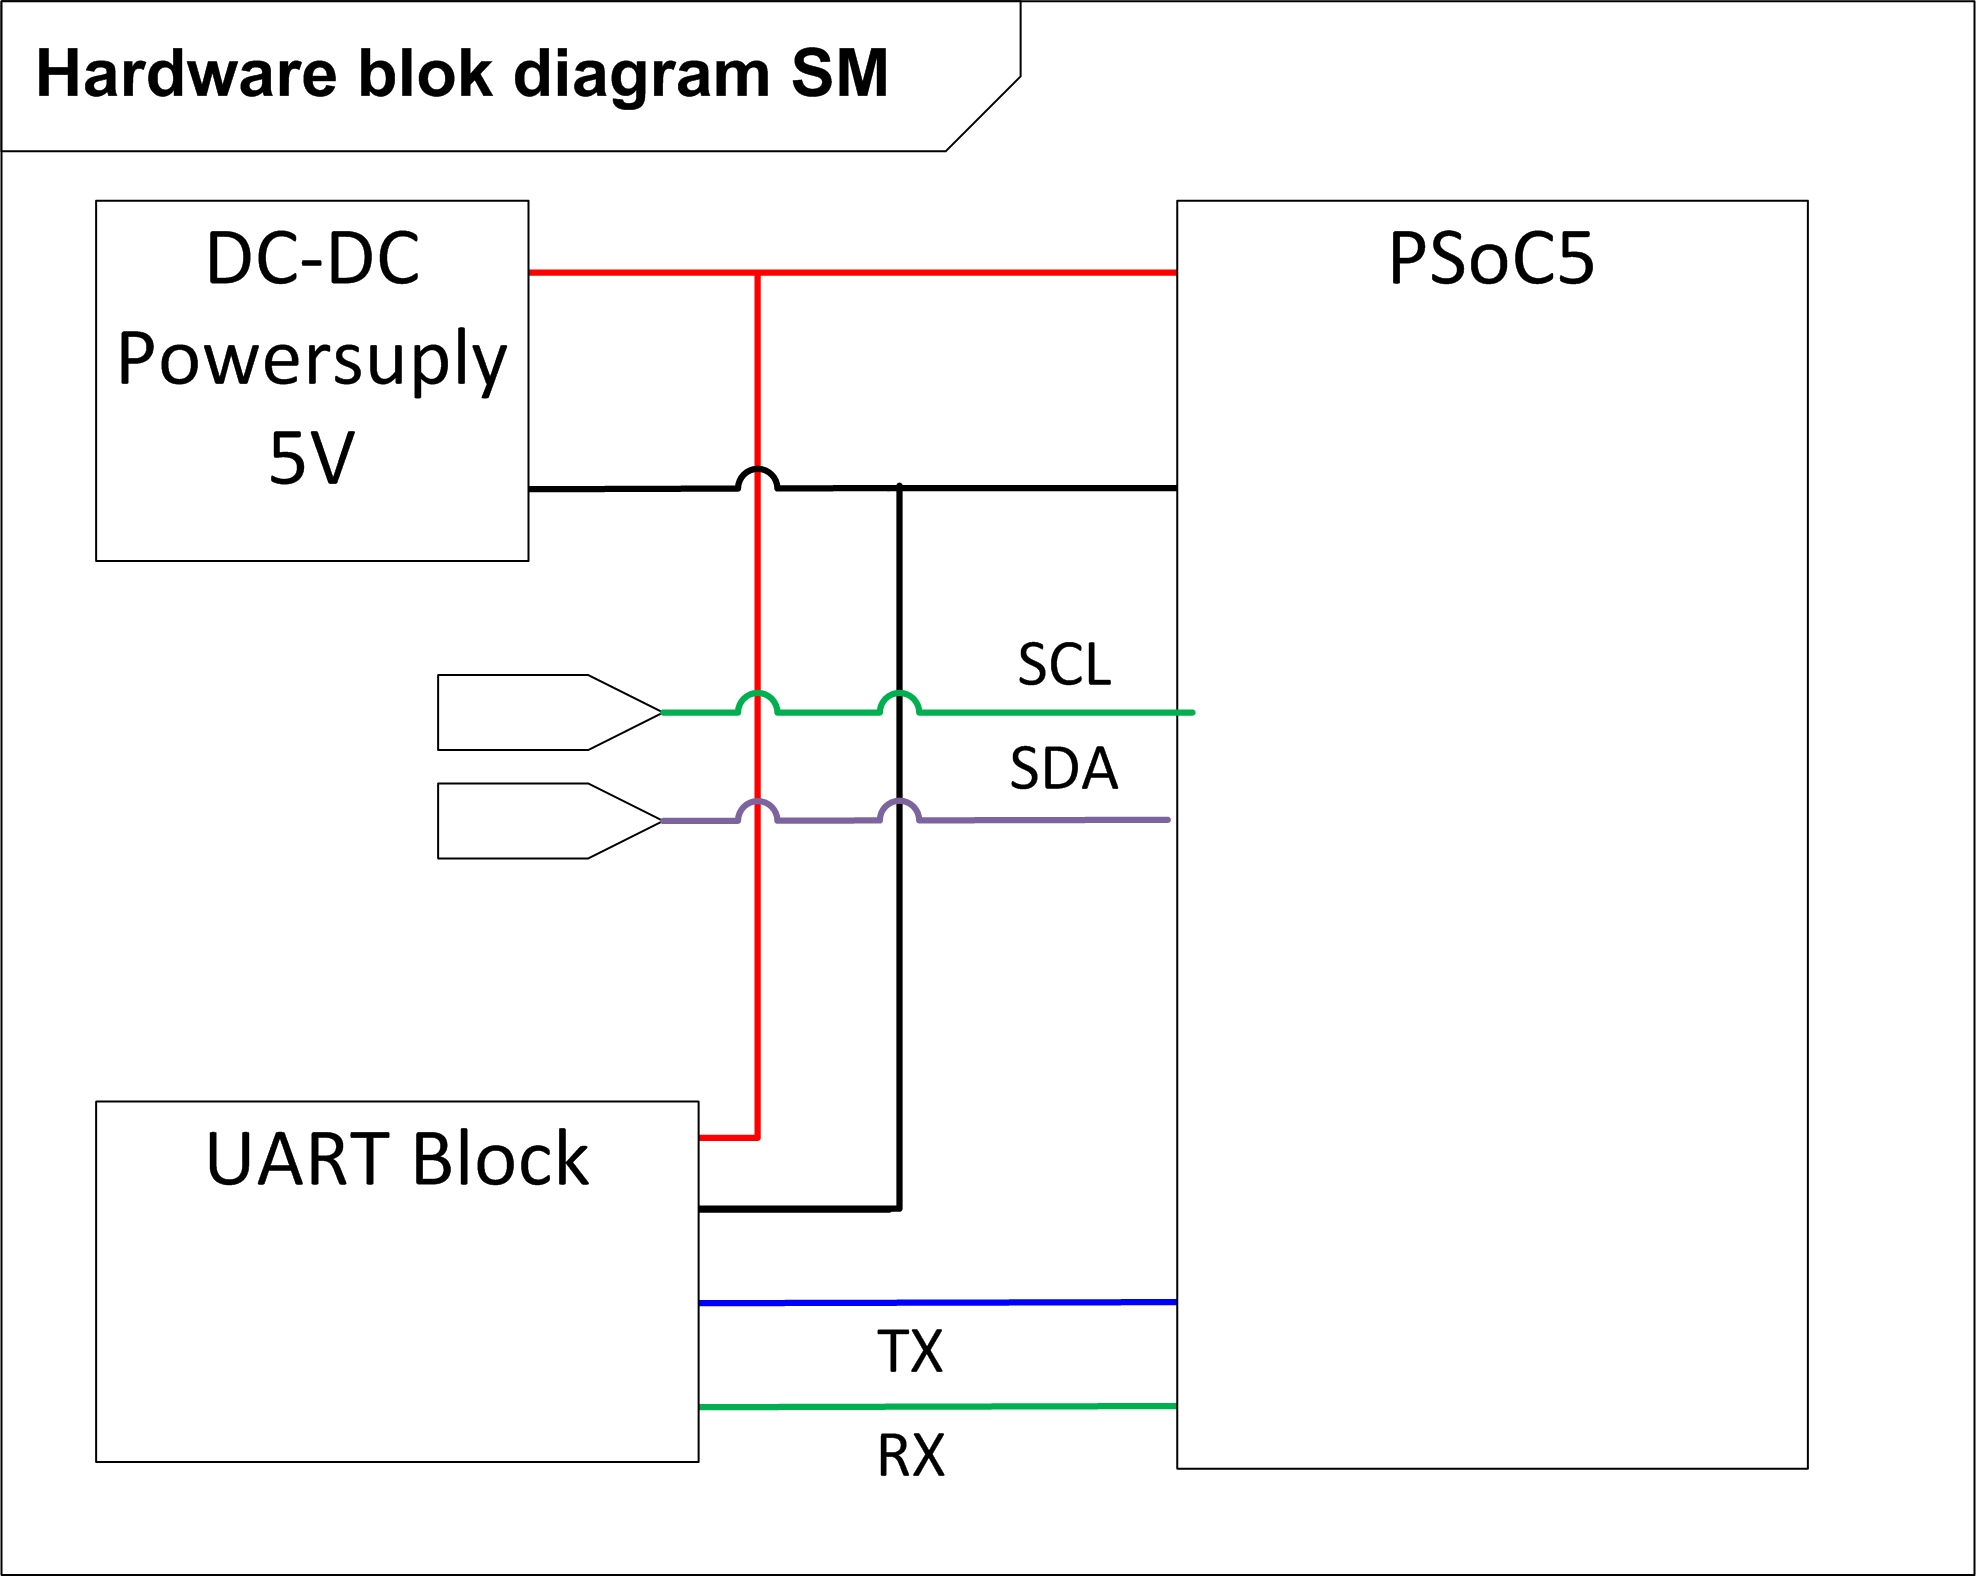
\includegraphics[width=0.5\textwidth]{billeder/SMHardware}
\caption{Overordnet blokdiagram for SM hardware}
\label{fig:HWSM}
\end{figure}
\subsection{Blokke}
Nedenfor beskrives de enkelte blokke illustreret på \textit{Figur~\ref{fig:HWSM}}
\subsubsection{PSoC5}
PSoC'en er den centrale del af VBTE'en og står for styringen af hele VBTE'en. Den består af:
\begin{itemize}
\item MicroController
\item I2C
\item Delta-Sigma ADC
\item Controlregister
\item UART
\end{itemize}
PSoC'en er et færdigkøbt produkt og for detaljer om de enkelte blokke heri henvises der til databladet for PSoC5.
\subsubsection{DC-DC powersuply 5V}
Se powersuply afsnittet.
\subsubsection{UART}
UART-blokken består af en levelkonverter forbundet til et DB9 stik. Levelkonverteren er af typen ST3232.
%%%%%% Nedbrydning af blokke
\section{Nedbrydning af blokke}
Nedenfor følger nedbrydningen af de enkelte blokke med henblik på at designe de enkelte dele til systemet. Nedbrydningen sker for at gøre designet nemmere og mere overskueligt.
\subsection{PSoC5}
På \textit{Figur~\ref{fig:HWPSoCSM}} ses  HW-designet internt på PSoC'en. De enkelte blokke bliver beskrevet efterfølgende.
\begin{figure}[H]
\centering
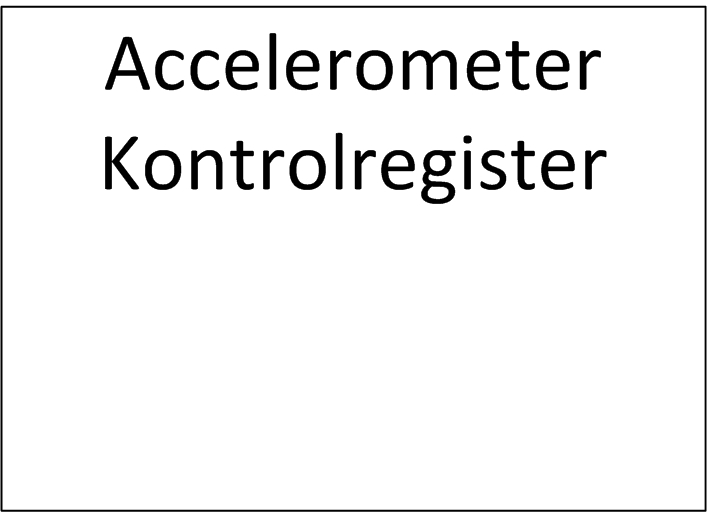
\includegraphics[width=0.7\textwidth]{billeder/SMPSoCblock}
\caption{PSoC5 blokdiagram}
\label{fig:HWPSoCSM}
\end{figure}
\subsubsection{Signalbeskrivelser:}
For signalbeskrivelser se \textit{tabel~\ref{table:PSoCSignalerSM}}
\begin{table}[H]
\begin{tabular}{|p{3cm}|p{3cm}|p{3cm}|p{4.5cm}|} \hline
\cellcolor[gray]{0.85}Signal navn& \cellcolor[gray]{0.85}Type &\cellcolor[gray]{0.85}Spænding&\cellcolor[gray]{0.85}Beskrivelse\\ \hline
TX & Analog & $\sim$0V til $\sim$5V & TX ud til UARTblokken.\\ \hline
RX & Analog & $\sim$0V til $\sim$5V & RX ud til UARTblokken \\ \hline
SDA & Digitalt & $\sim$0V til $\sim$5V & Et digitalt signal mellem VBTE og SM hvor I2C data læses fra.\\ \hline
SCL & Digitalt & $\sim$0V til $\sim$5V & Digitalt clocksignal til I2C.\\ \hline
\end{tabular}
\caption{Tabel over signaler i PSoC blokken}
\label{table:PSoCSignalerSM}
\end{table}
\subsubsection{Blokbeskrivelser:}
\subsubsection{Hældningssensor}
Hældningssensorblokken står for at modtage og konvertere værdier fra hældningssensoren til en integer der er forståelig for vores digitale elektronik. Konverteringen skal se med en A/D konverter med en høj nok opløsning til at måle det udsving angivet i kravspecifikationen.
\subsubsection{UART}
naha
\subsubsection{Accelerometer Controlregister}
hest
\subsubsection{I2C kreds}
I2C kredsen skal stå for I2C interfacet mellem SM og KI. I2C protokollen kører 5V og med pull-up modstande. I2C'en benytter standard I2C protokol, og for yderligere info om data henvises der til \textit{Systemarkitektur/protokoller/I2C}.
%%%%%%%%% UART controller %%%%%%%%%%%%%
\subsection{UART}
